\documentclass[11pt]{article}
\usepackage[margin=1in]{geometry}
\usepackage{booktabs}
\usepackage{graphicx}
\usepackage{float}
\begin{document}
\section*{Supplementary Step 6 Visualization Report}
\subsection*{Overview}
\begin{tabular}{p{0.36\linewidth}p{0.54\linewidth}}
\toprule
Metric & Value\\
\midrule
Representative geometry session & PID001 / 2025-11-06\_008\\
Included participant-sessions from Step 6 & 36\\
Included questions in Step 6 trial table & 30\\
Abstract onset-locked epochs used & 539\\
Concrete onset-locked epochs used & 536\\
Epoch window & -3.5 s to 13.2 s around question onset\\
Baseline & -2.0 s to 0.0 s\\
Long-channel montage used in descriptive plots & 22 pairs (44 chromophore channels)\\
Primary Step 6 adjusted p-value & 0.052102\\
\bottomrule
\end{tabular}
\paragraph{Adaptation note.} This report reuses the same supplementary visualization family created for Step~5, but anchors it explicitly to the Step~6 trial-model table. Because Step~6 freezes the Step~5 cohort and outcome definition, the onset-locked descriptive plots shown here are based on the same included trial set that feeds the covariate-adjusted mixed-effects models.
\paragraph{Rendering note.} As in the earlier supplementary visualization reports, the sensor-geometry figure uses the participant digitization point cloud plus source, detector, channel, and pair geometry rather than an fsaverage brain-surface rendering, because the local \texttt{pyvista}/\texttt{fsaverage} stack is not available in this environment.
\subsection*{Step 6 Main Figures Reused}
\begin{figure}[H]
\centering
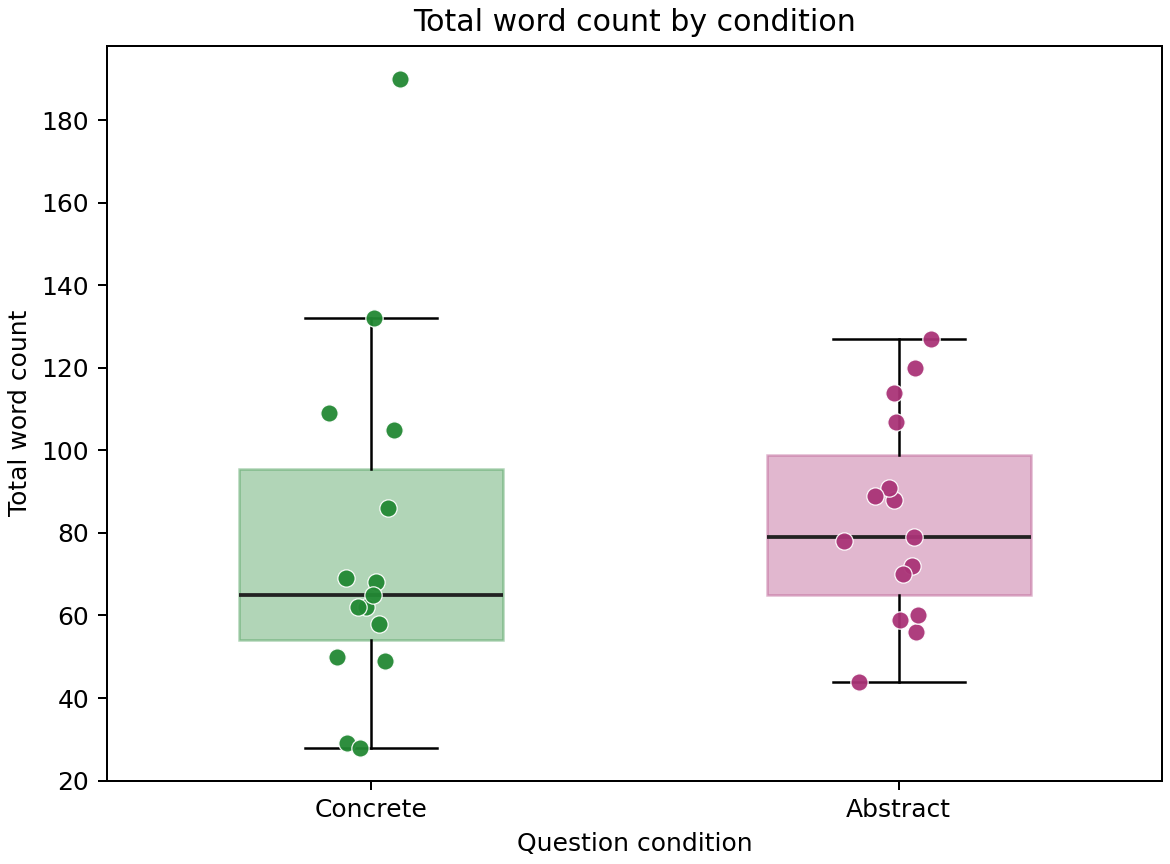
\includegraphics[width=0.48\linewidth]{../../figures/step6/wordcount_by_condition.png}
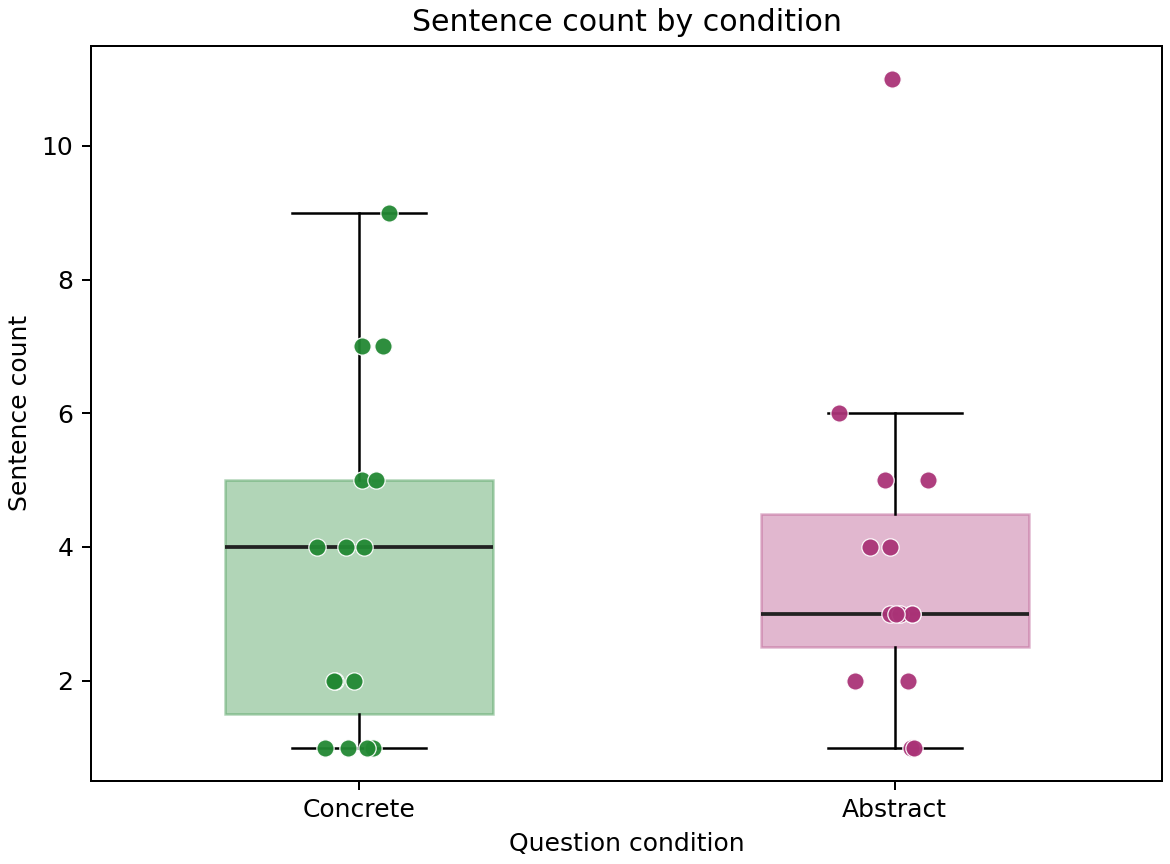
\includegraphics[width=0.48\linewidth]{../../figures/step6/sentencecount_by_condition.png}
\caption{Step~6 item-level balance plots for total word count and sentence count.}
\end{figure}
\begin{figure}[H]
\centering
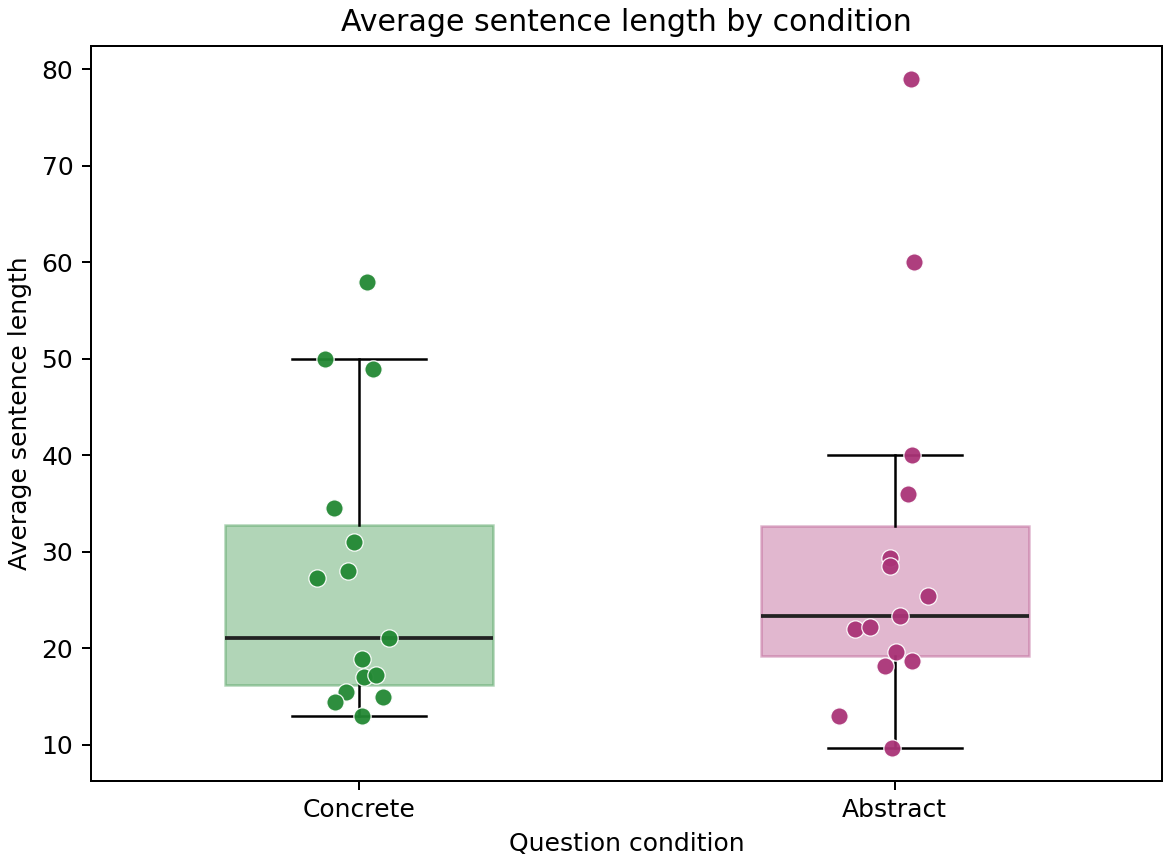
\includegraphics[width=0.48\linewidth]{../../figures/step6/sentencelength_by_condition.png}
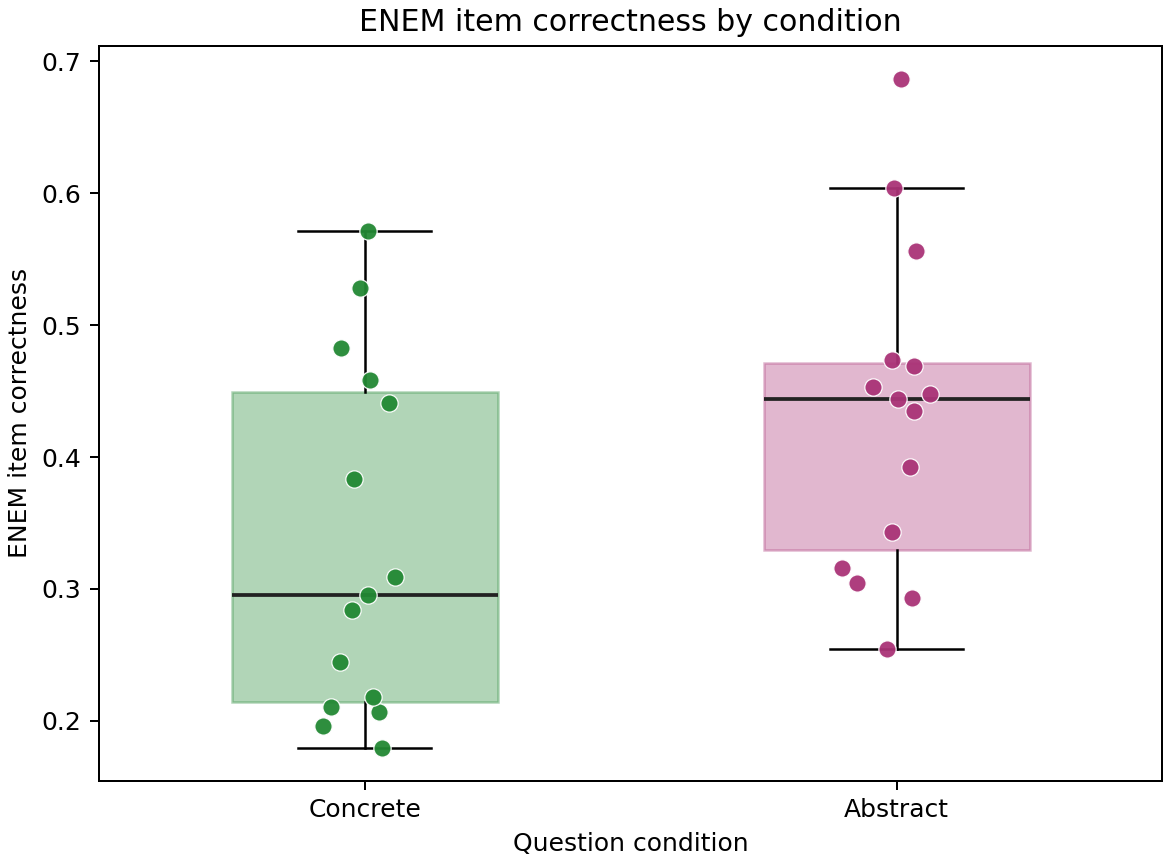
\includegraphics[width=0.48\linewidth]{../../figures/step6/enem_correctness_by_condition.png}
\caption{Step~6 item-level balance plots for sentence length and ENEM item correctness.}
\end{figure}
\begin{figure}[H]
\centering
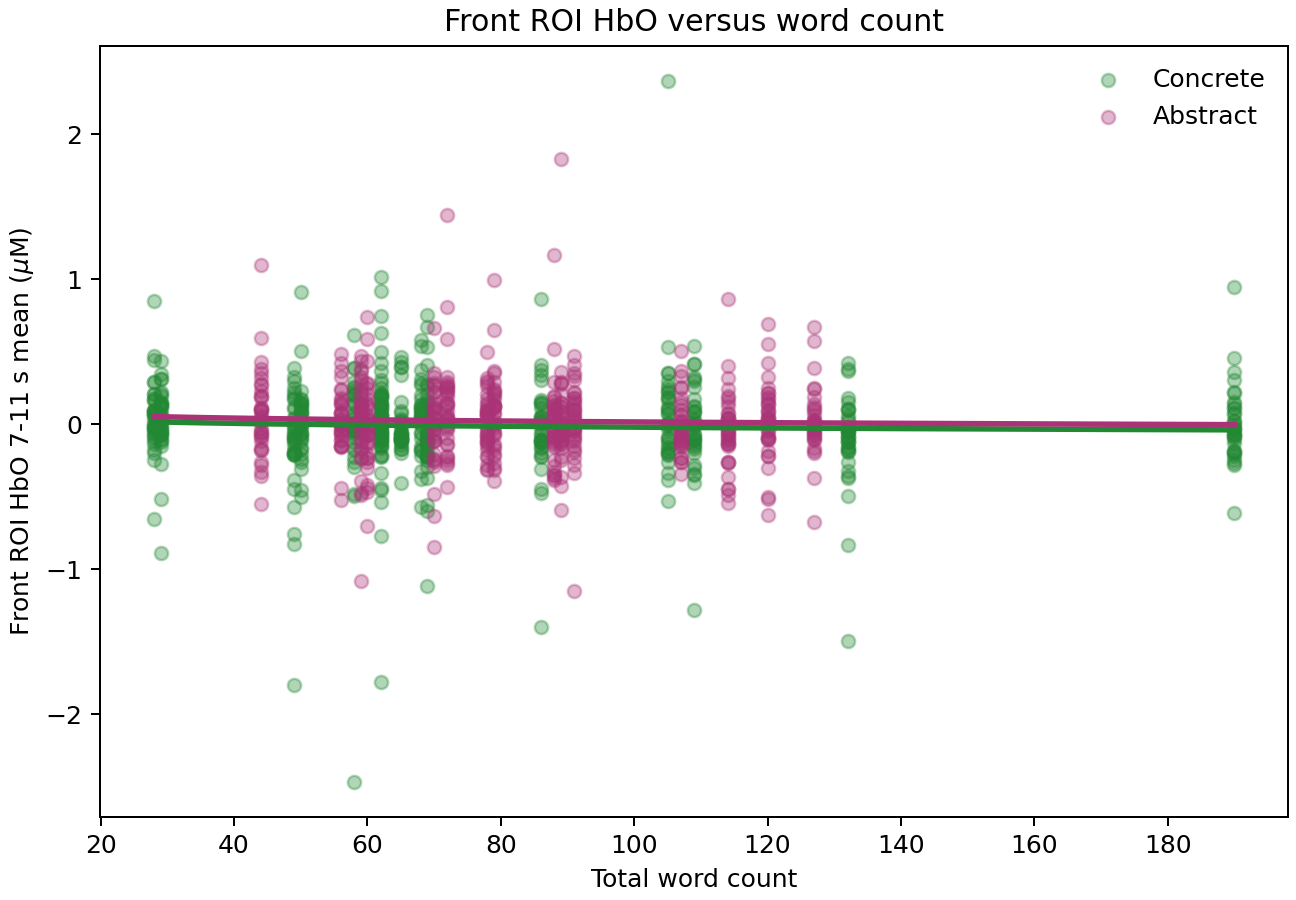
\includegraphics[width=0.48\linewidth]{../../figures/step6/front_roi_vs_wordcount_scatter.png}
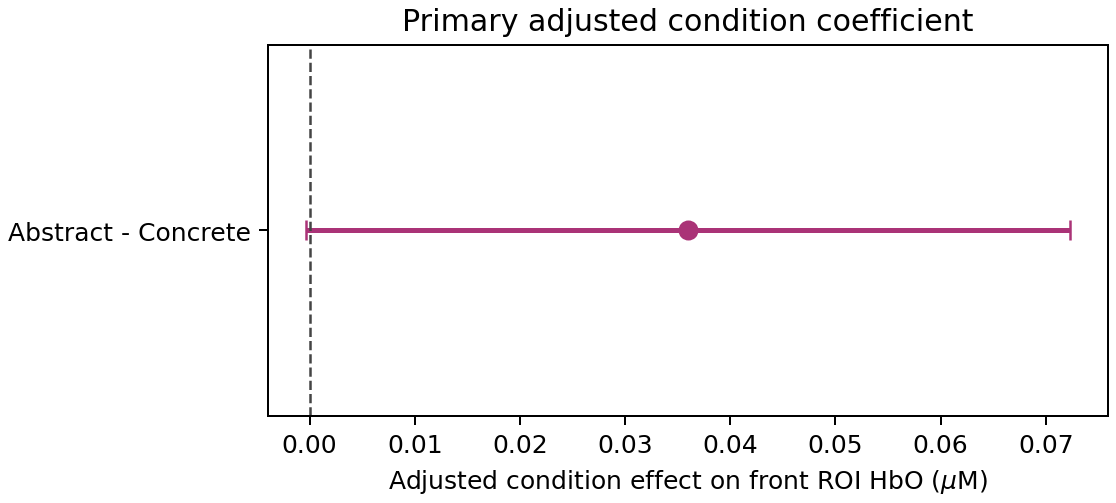
\includegraphics[width=0.48\linewidth]{../../figures/step6/front_roi_partial_effect_condition.png}
\caption{Step~6 scatter and partial-effect figures from the primary covariate-adjusted model.}
\end{figure}
\begin{figure}[H]
\centering
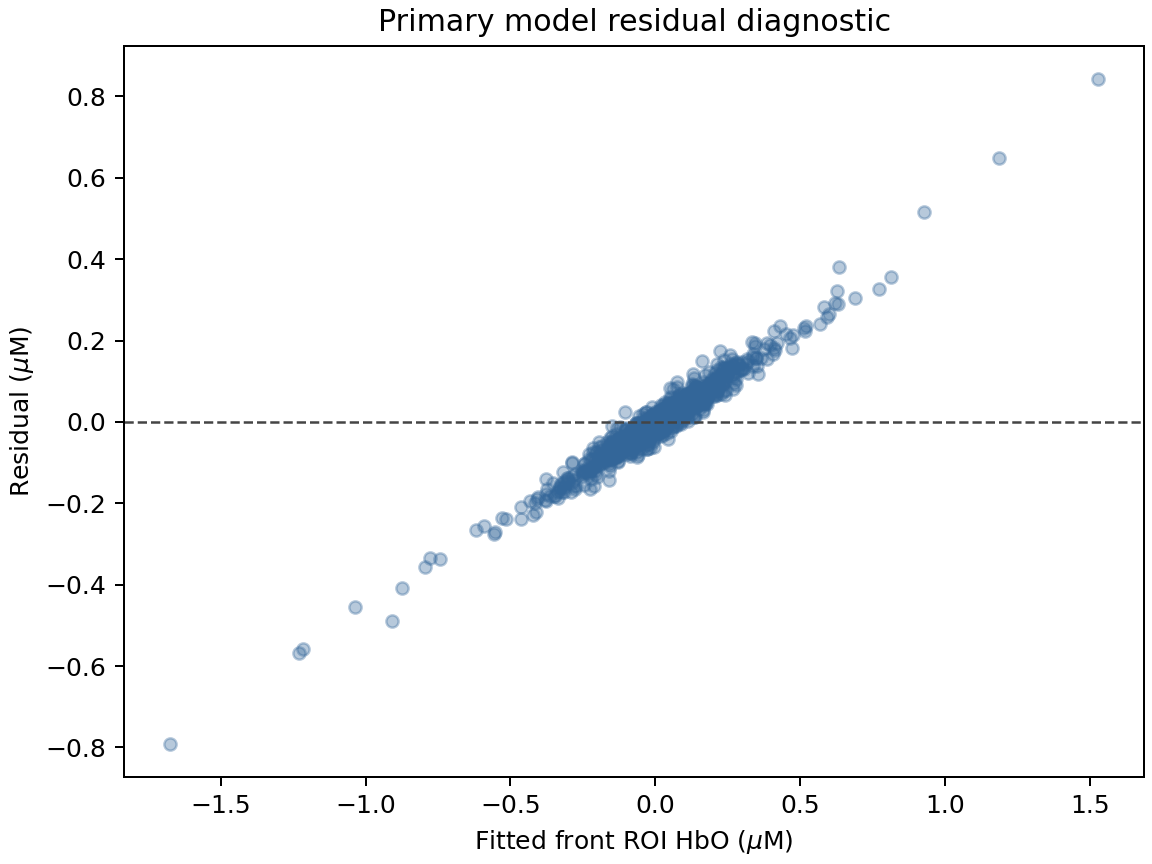
\includegraphics[width=0.48\linewidth]{../../figures/step6/model_residuals_primary.png}
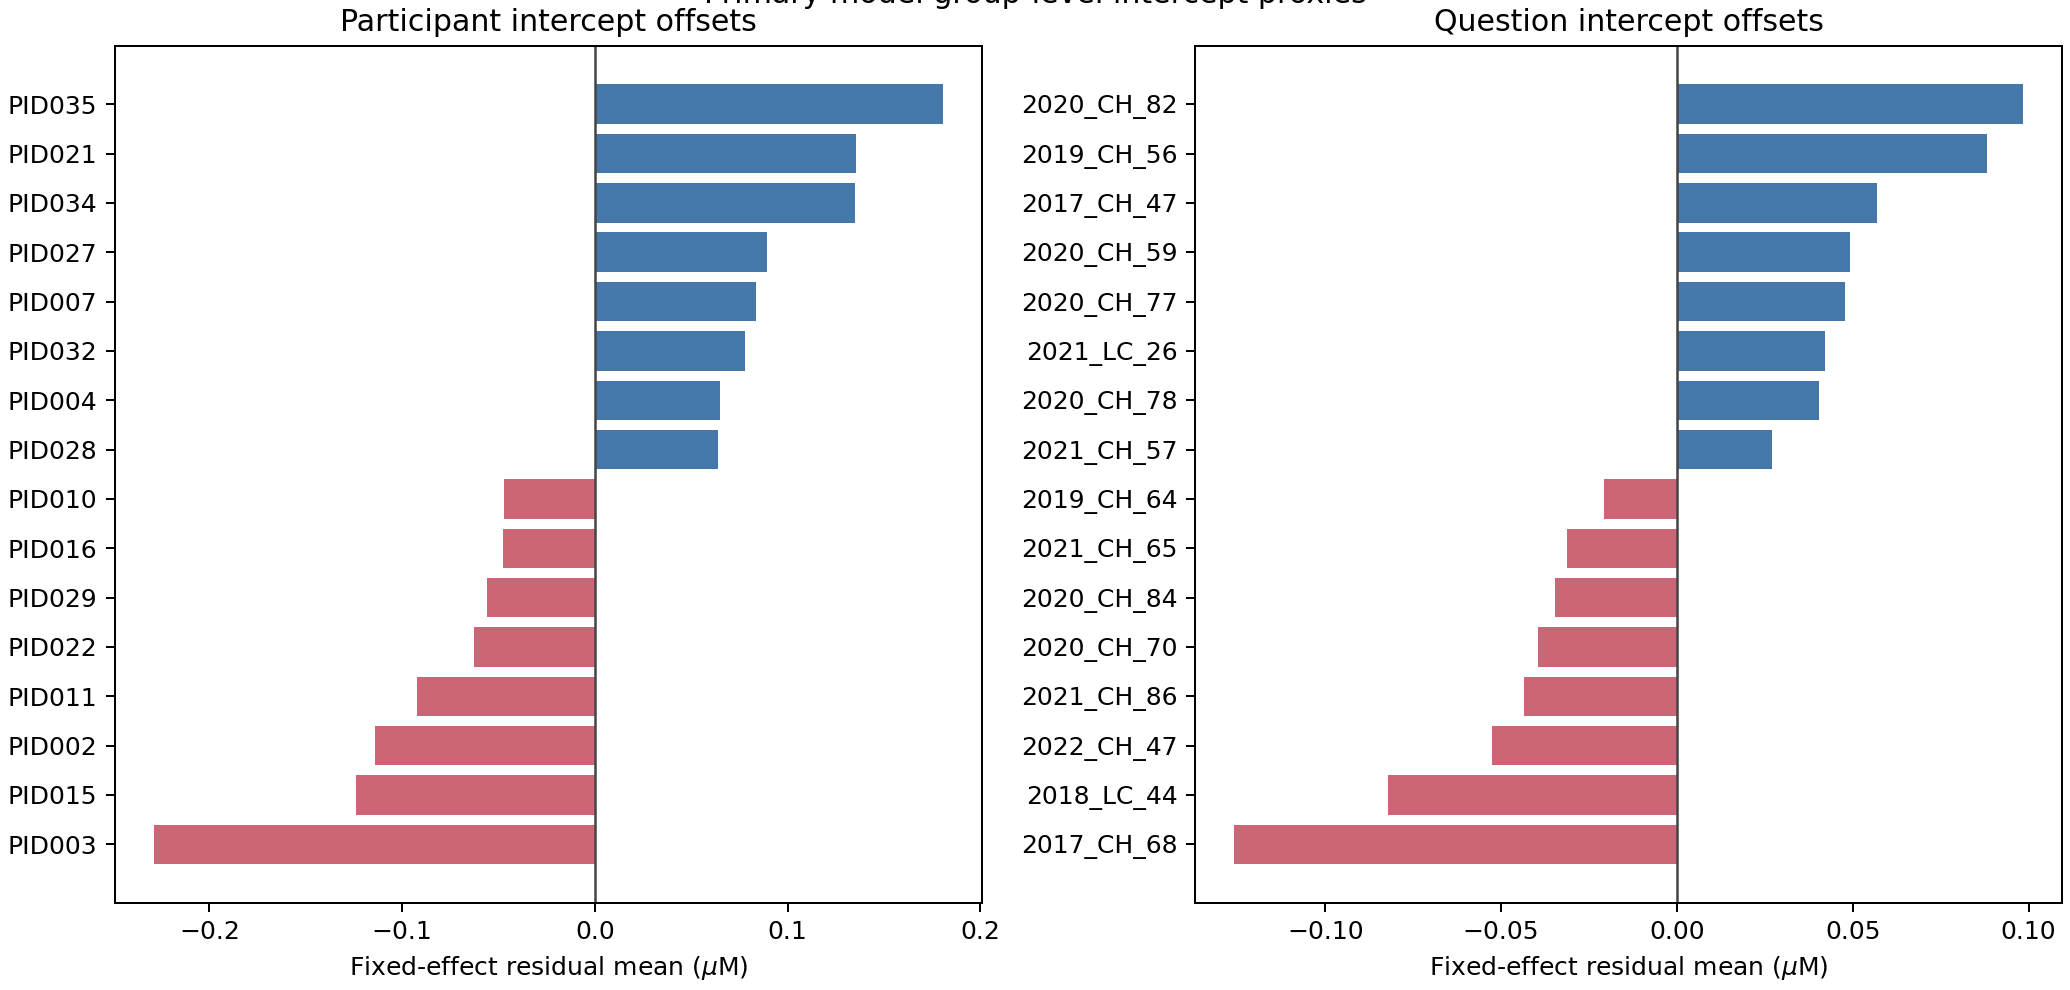
\includegraphics[width=0.48\linewidth]{../../figures/step6/model_random_intercepts.png}
\caption{Step~6 residual diagnostic and group-level intercept-proxy plots from the primary model.}
\end{figure}
\subsection*{Step 5-Style Supplementary Plots for Step 6}
\begin{figure}[H]
\centering
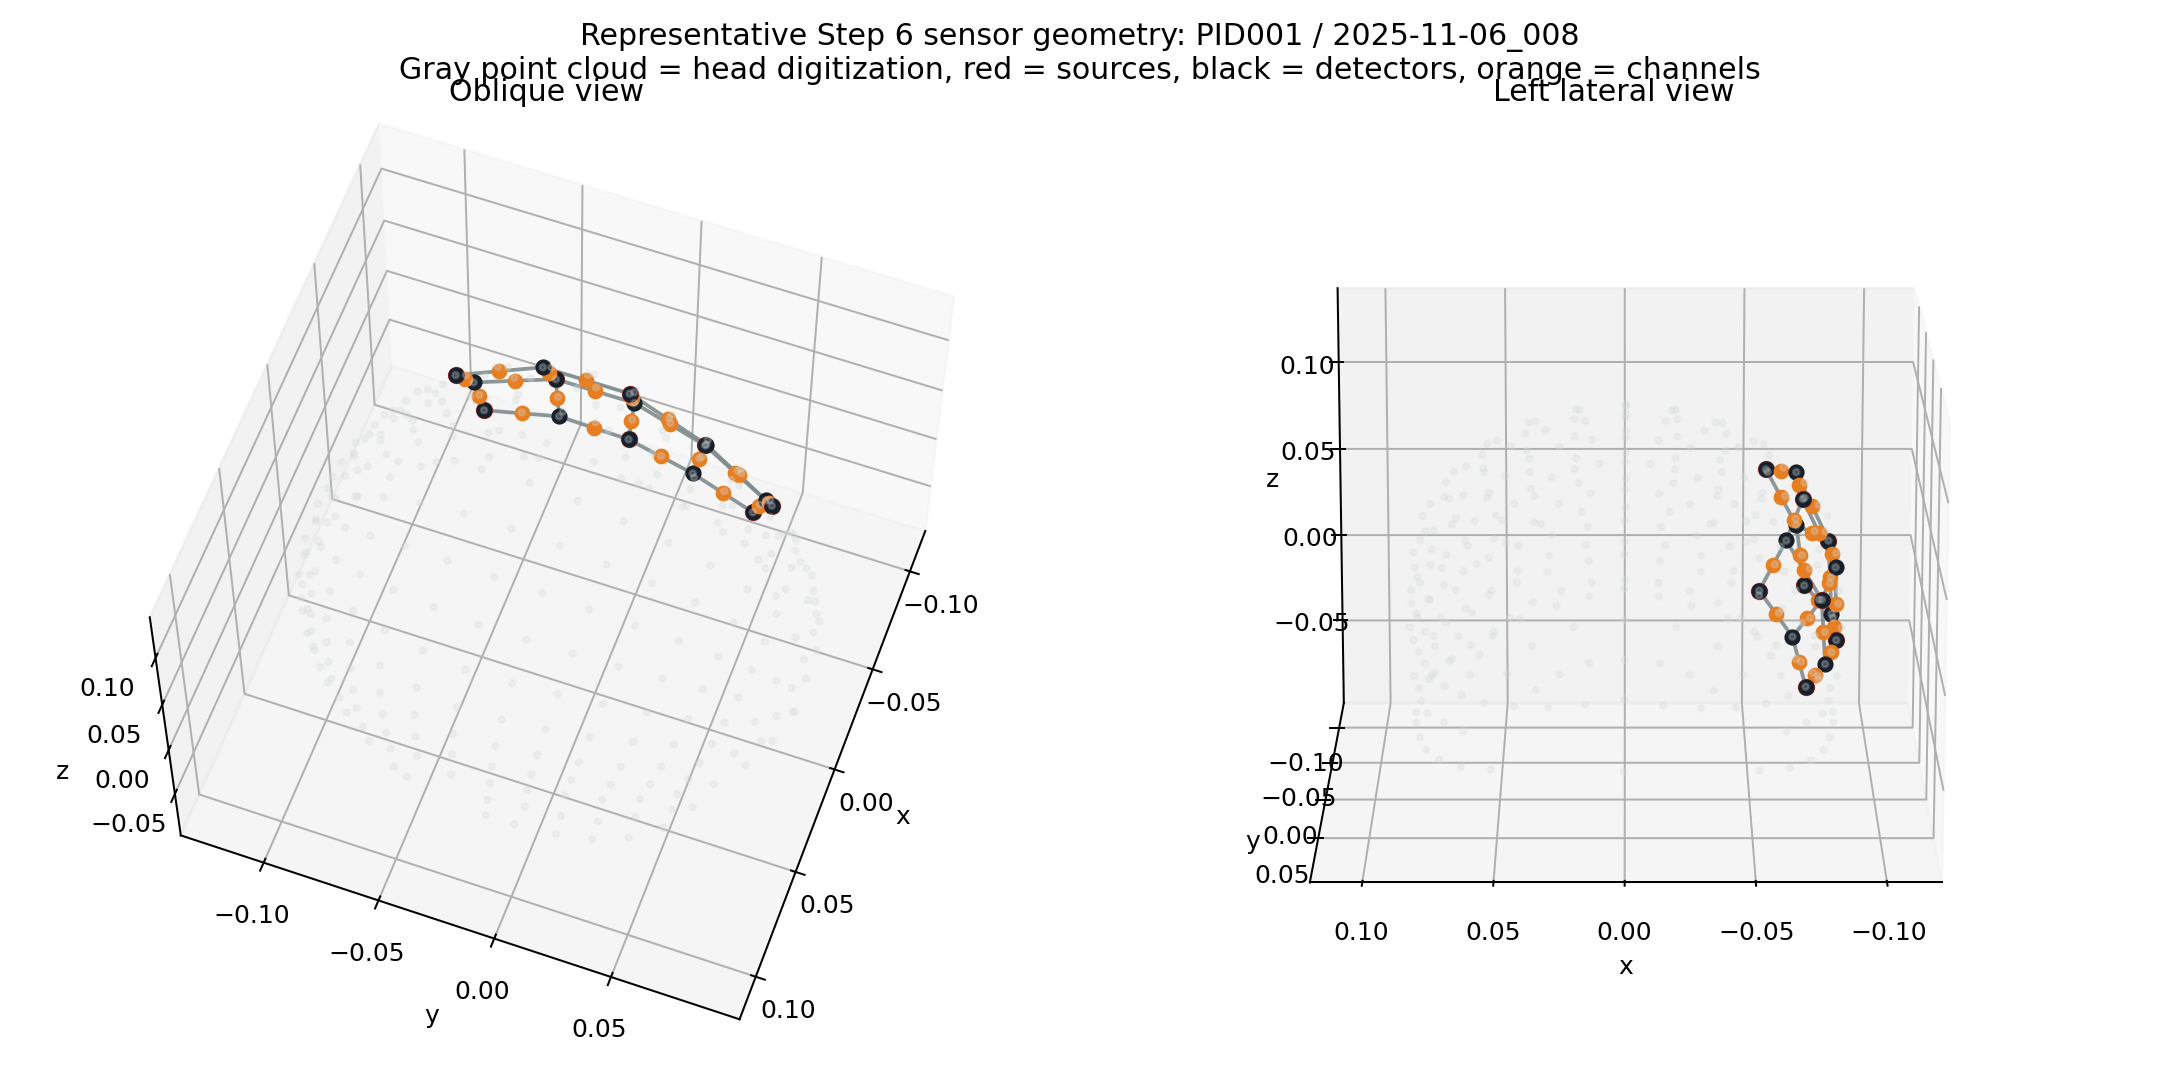
\includegraphics[width=0.95\linewidth]{../../figures/step6_visualization/representative_sensor_geometry.png}
\caption{Representative optode, channel, and source-detector-pair geometry for one Step~6 included participant-session. Short pairs are shown with dashed orange lines.}
\end{figure}
\begin{figure}[H]
\centering
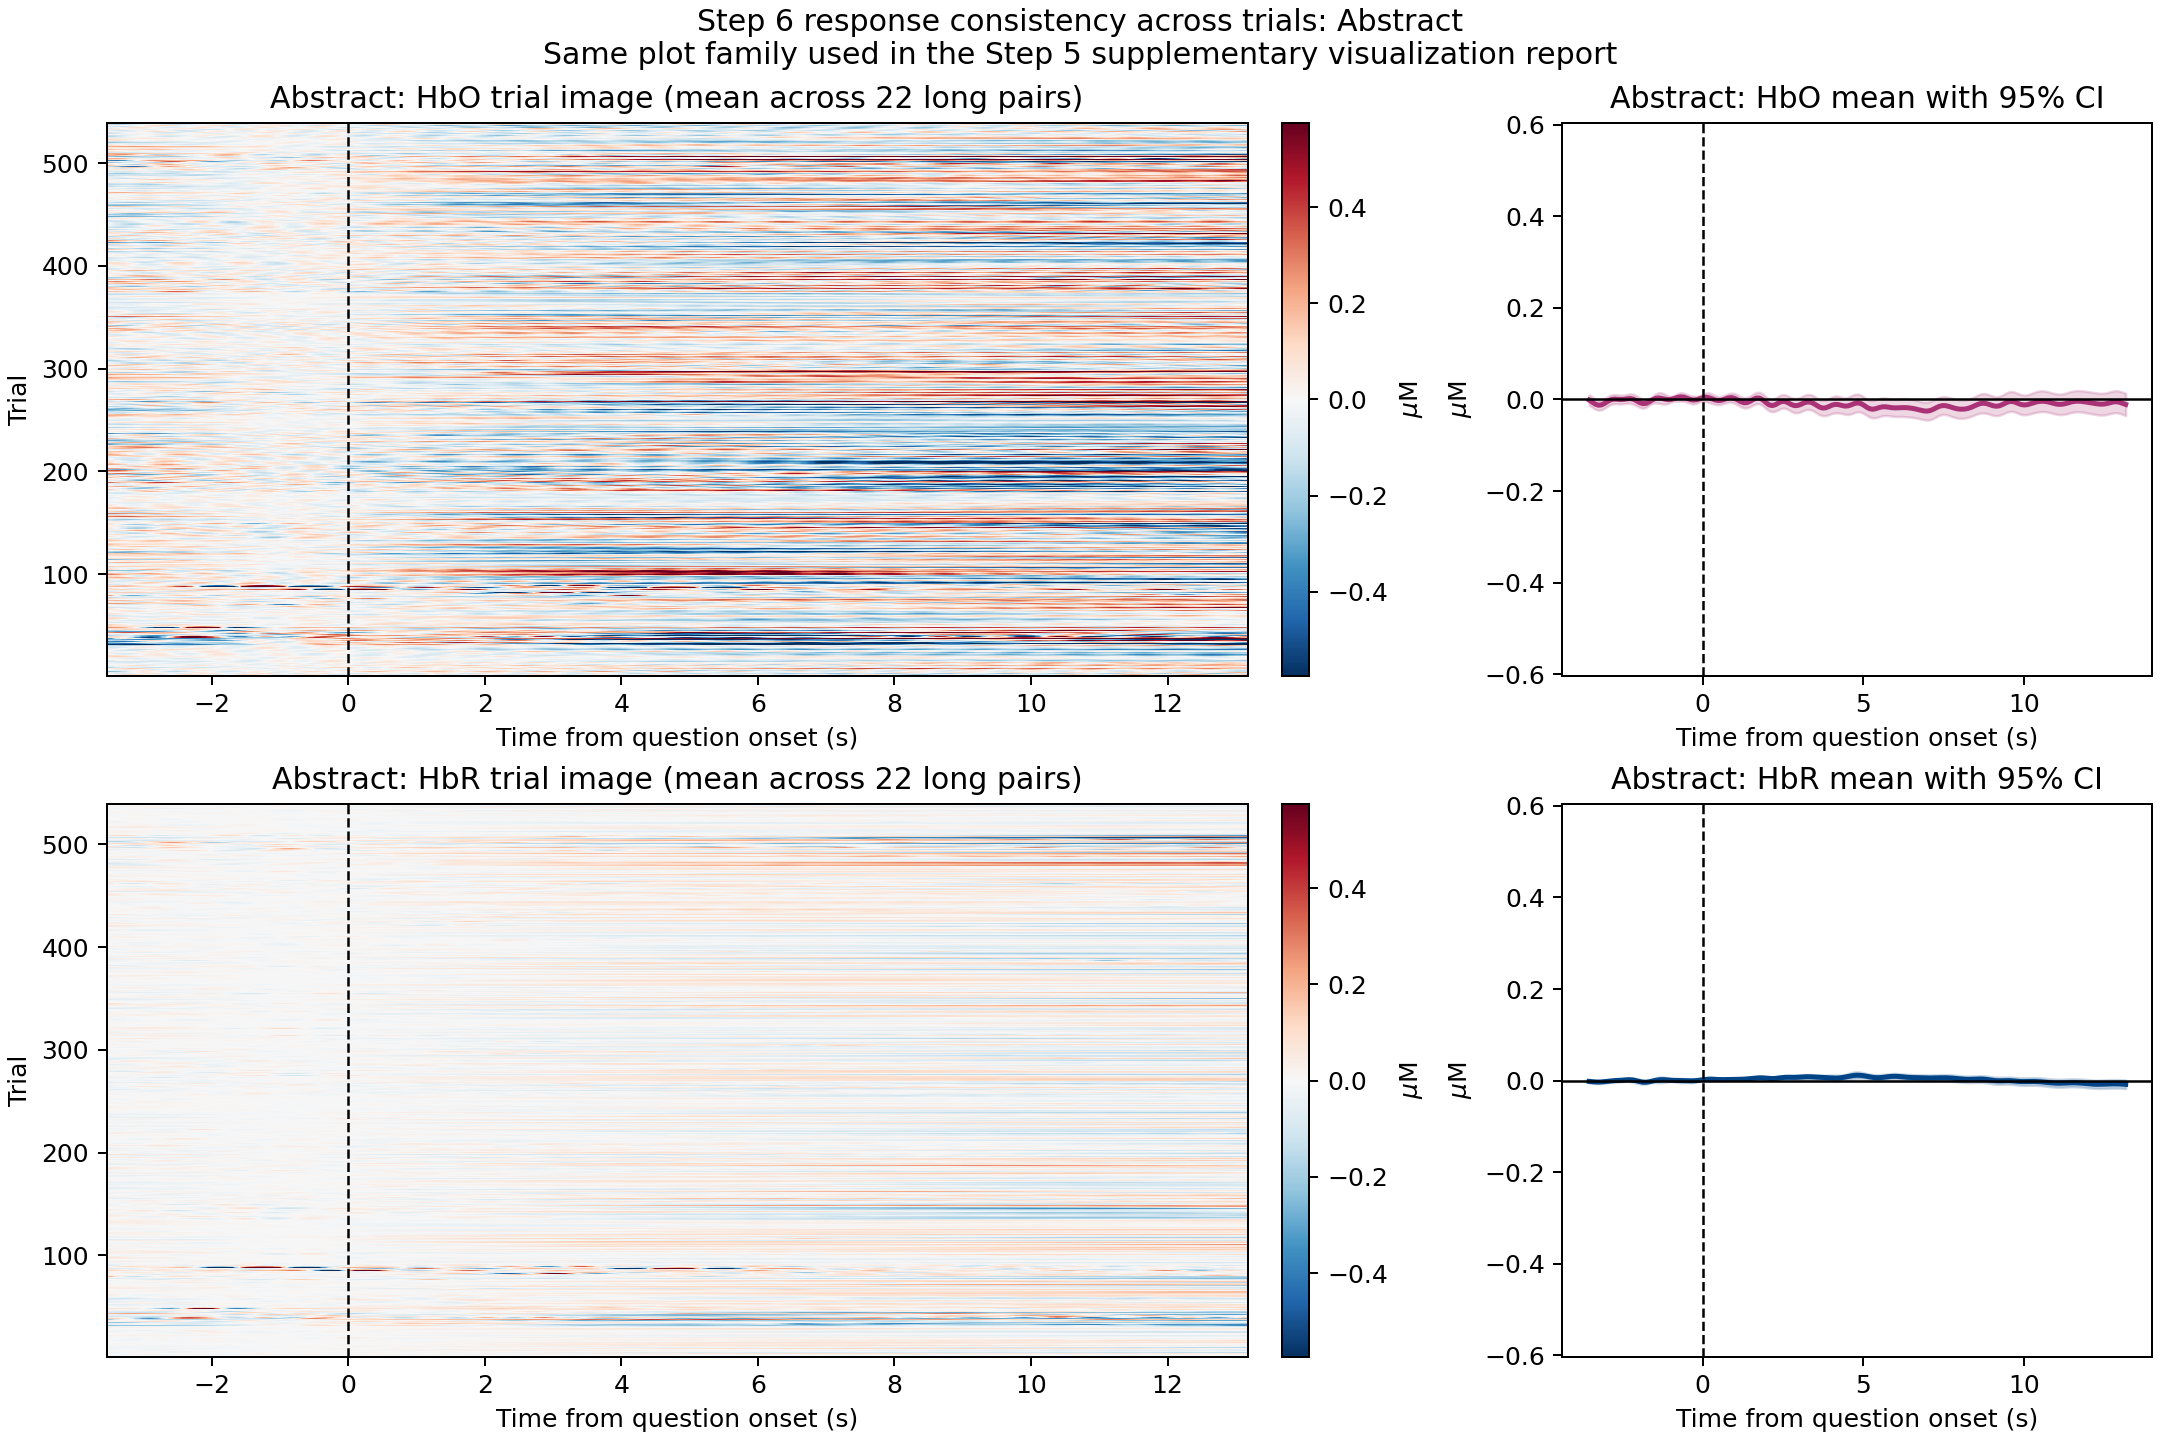
\includegraphics[width=0.48\linewidth]{../../figures/step6_visualization/abstract_trial_consistency.png}
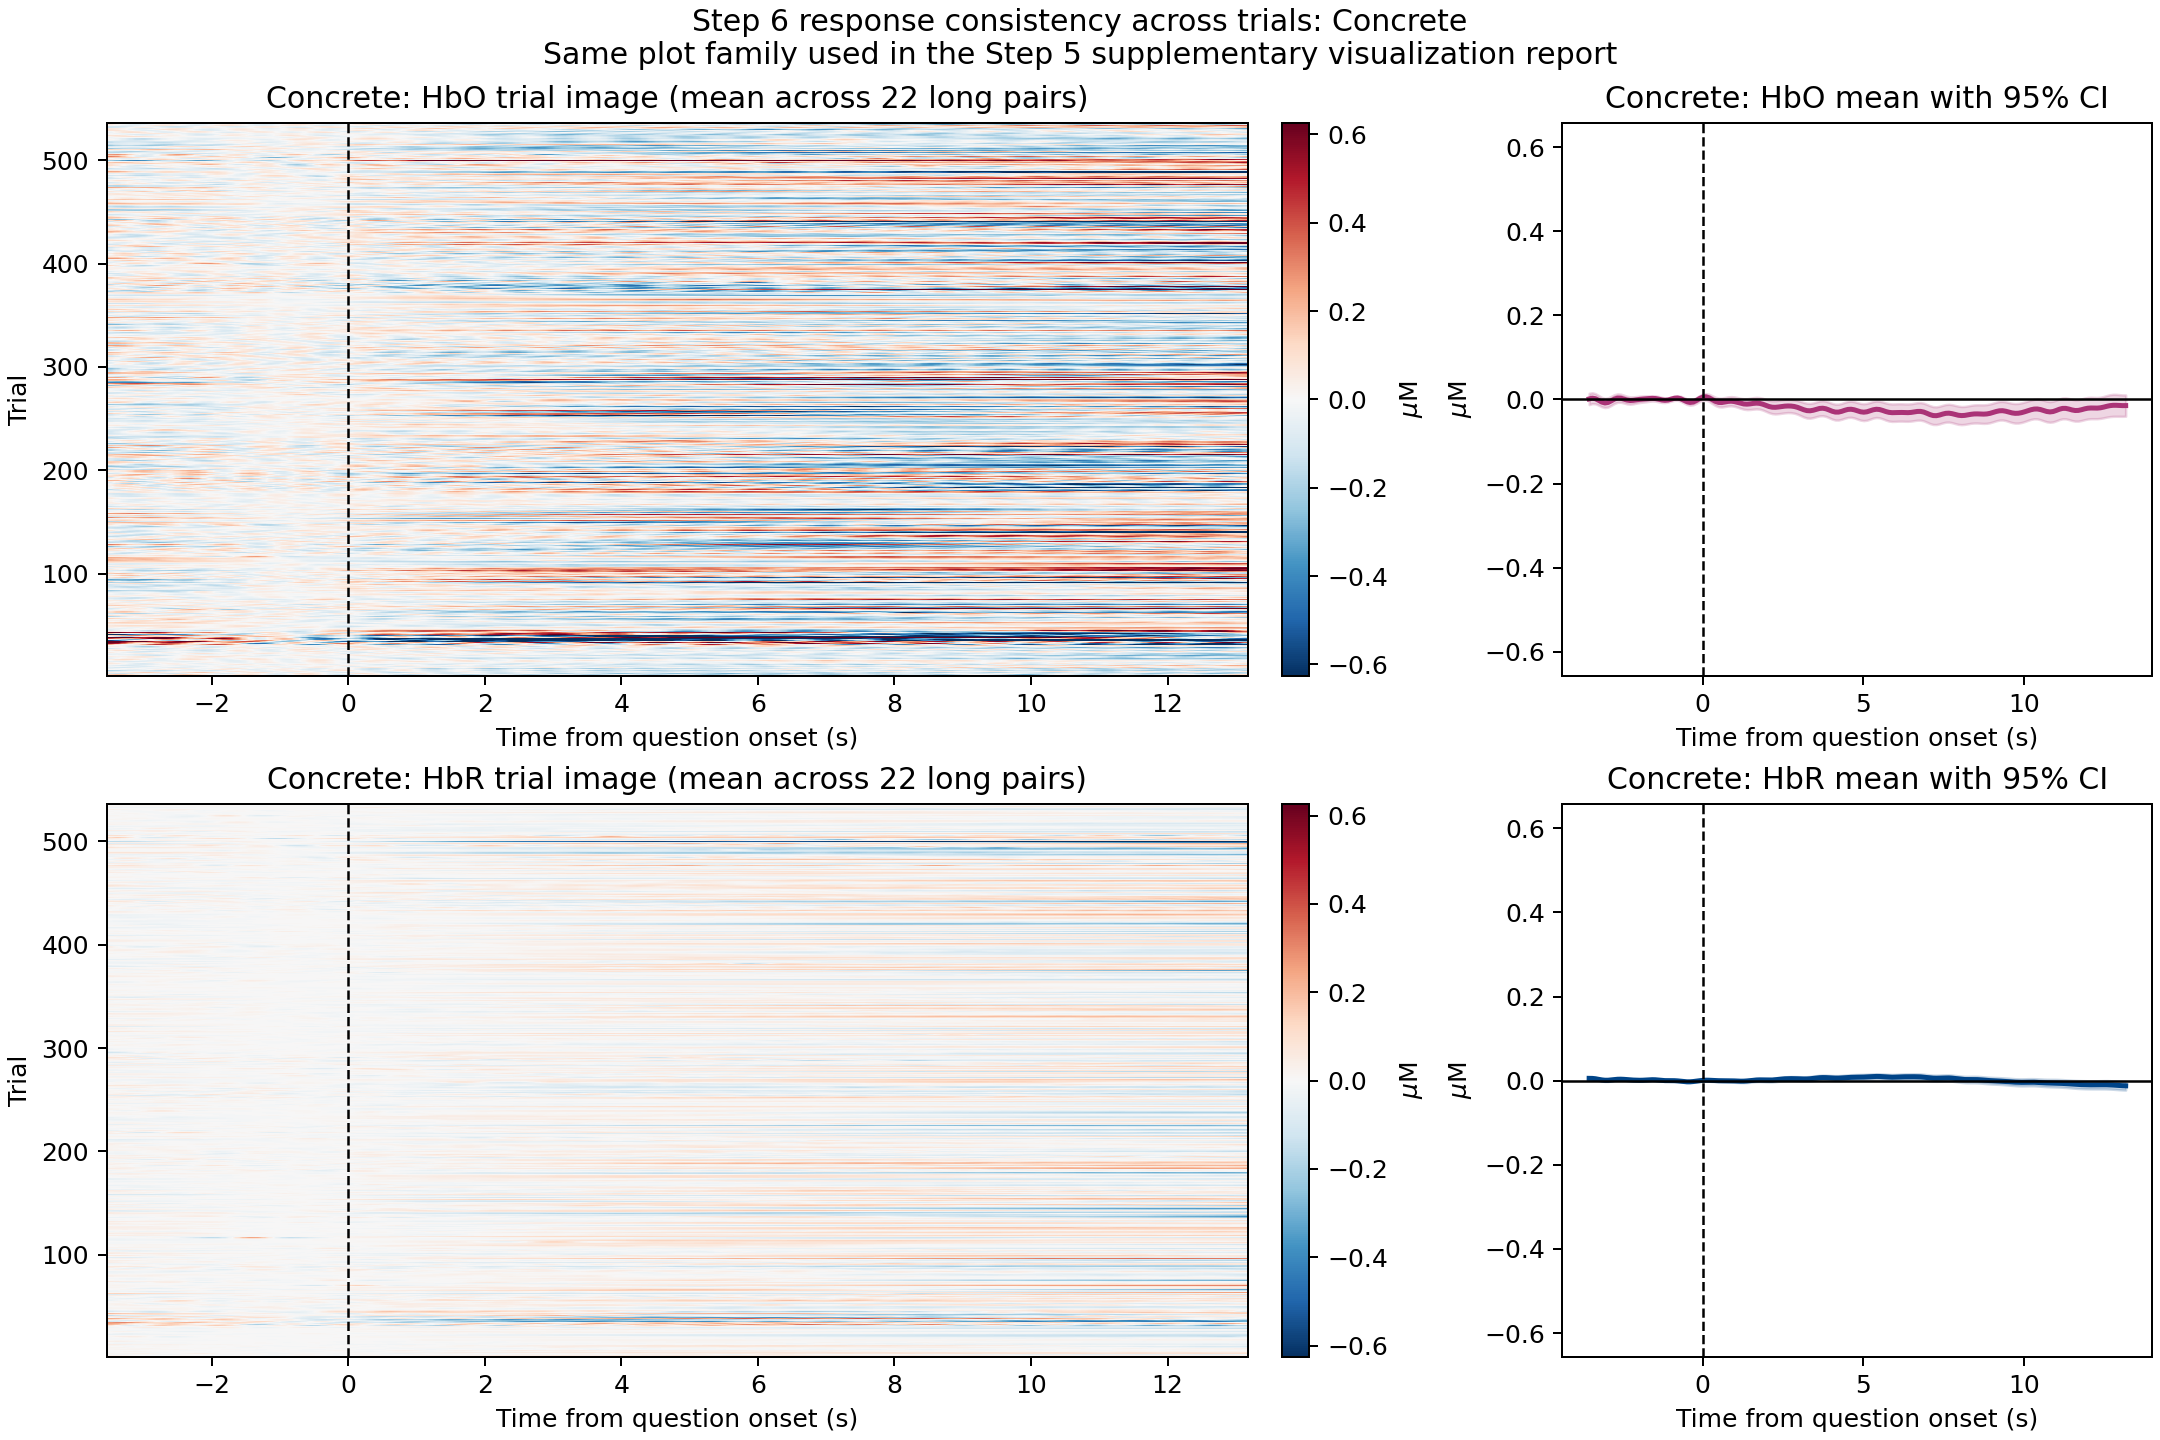
\includegraphics[width=0.48\linewidth]{../../figures/step6_visualization/concrete_trial_consistency.png}
\caption{Condition-adapted trial-consistency image plots for the Step~6 trial set.}
\end{figure}
\begin{figure}[H]
\centering
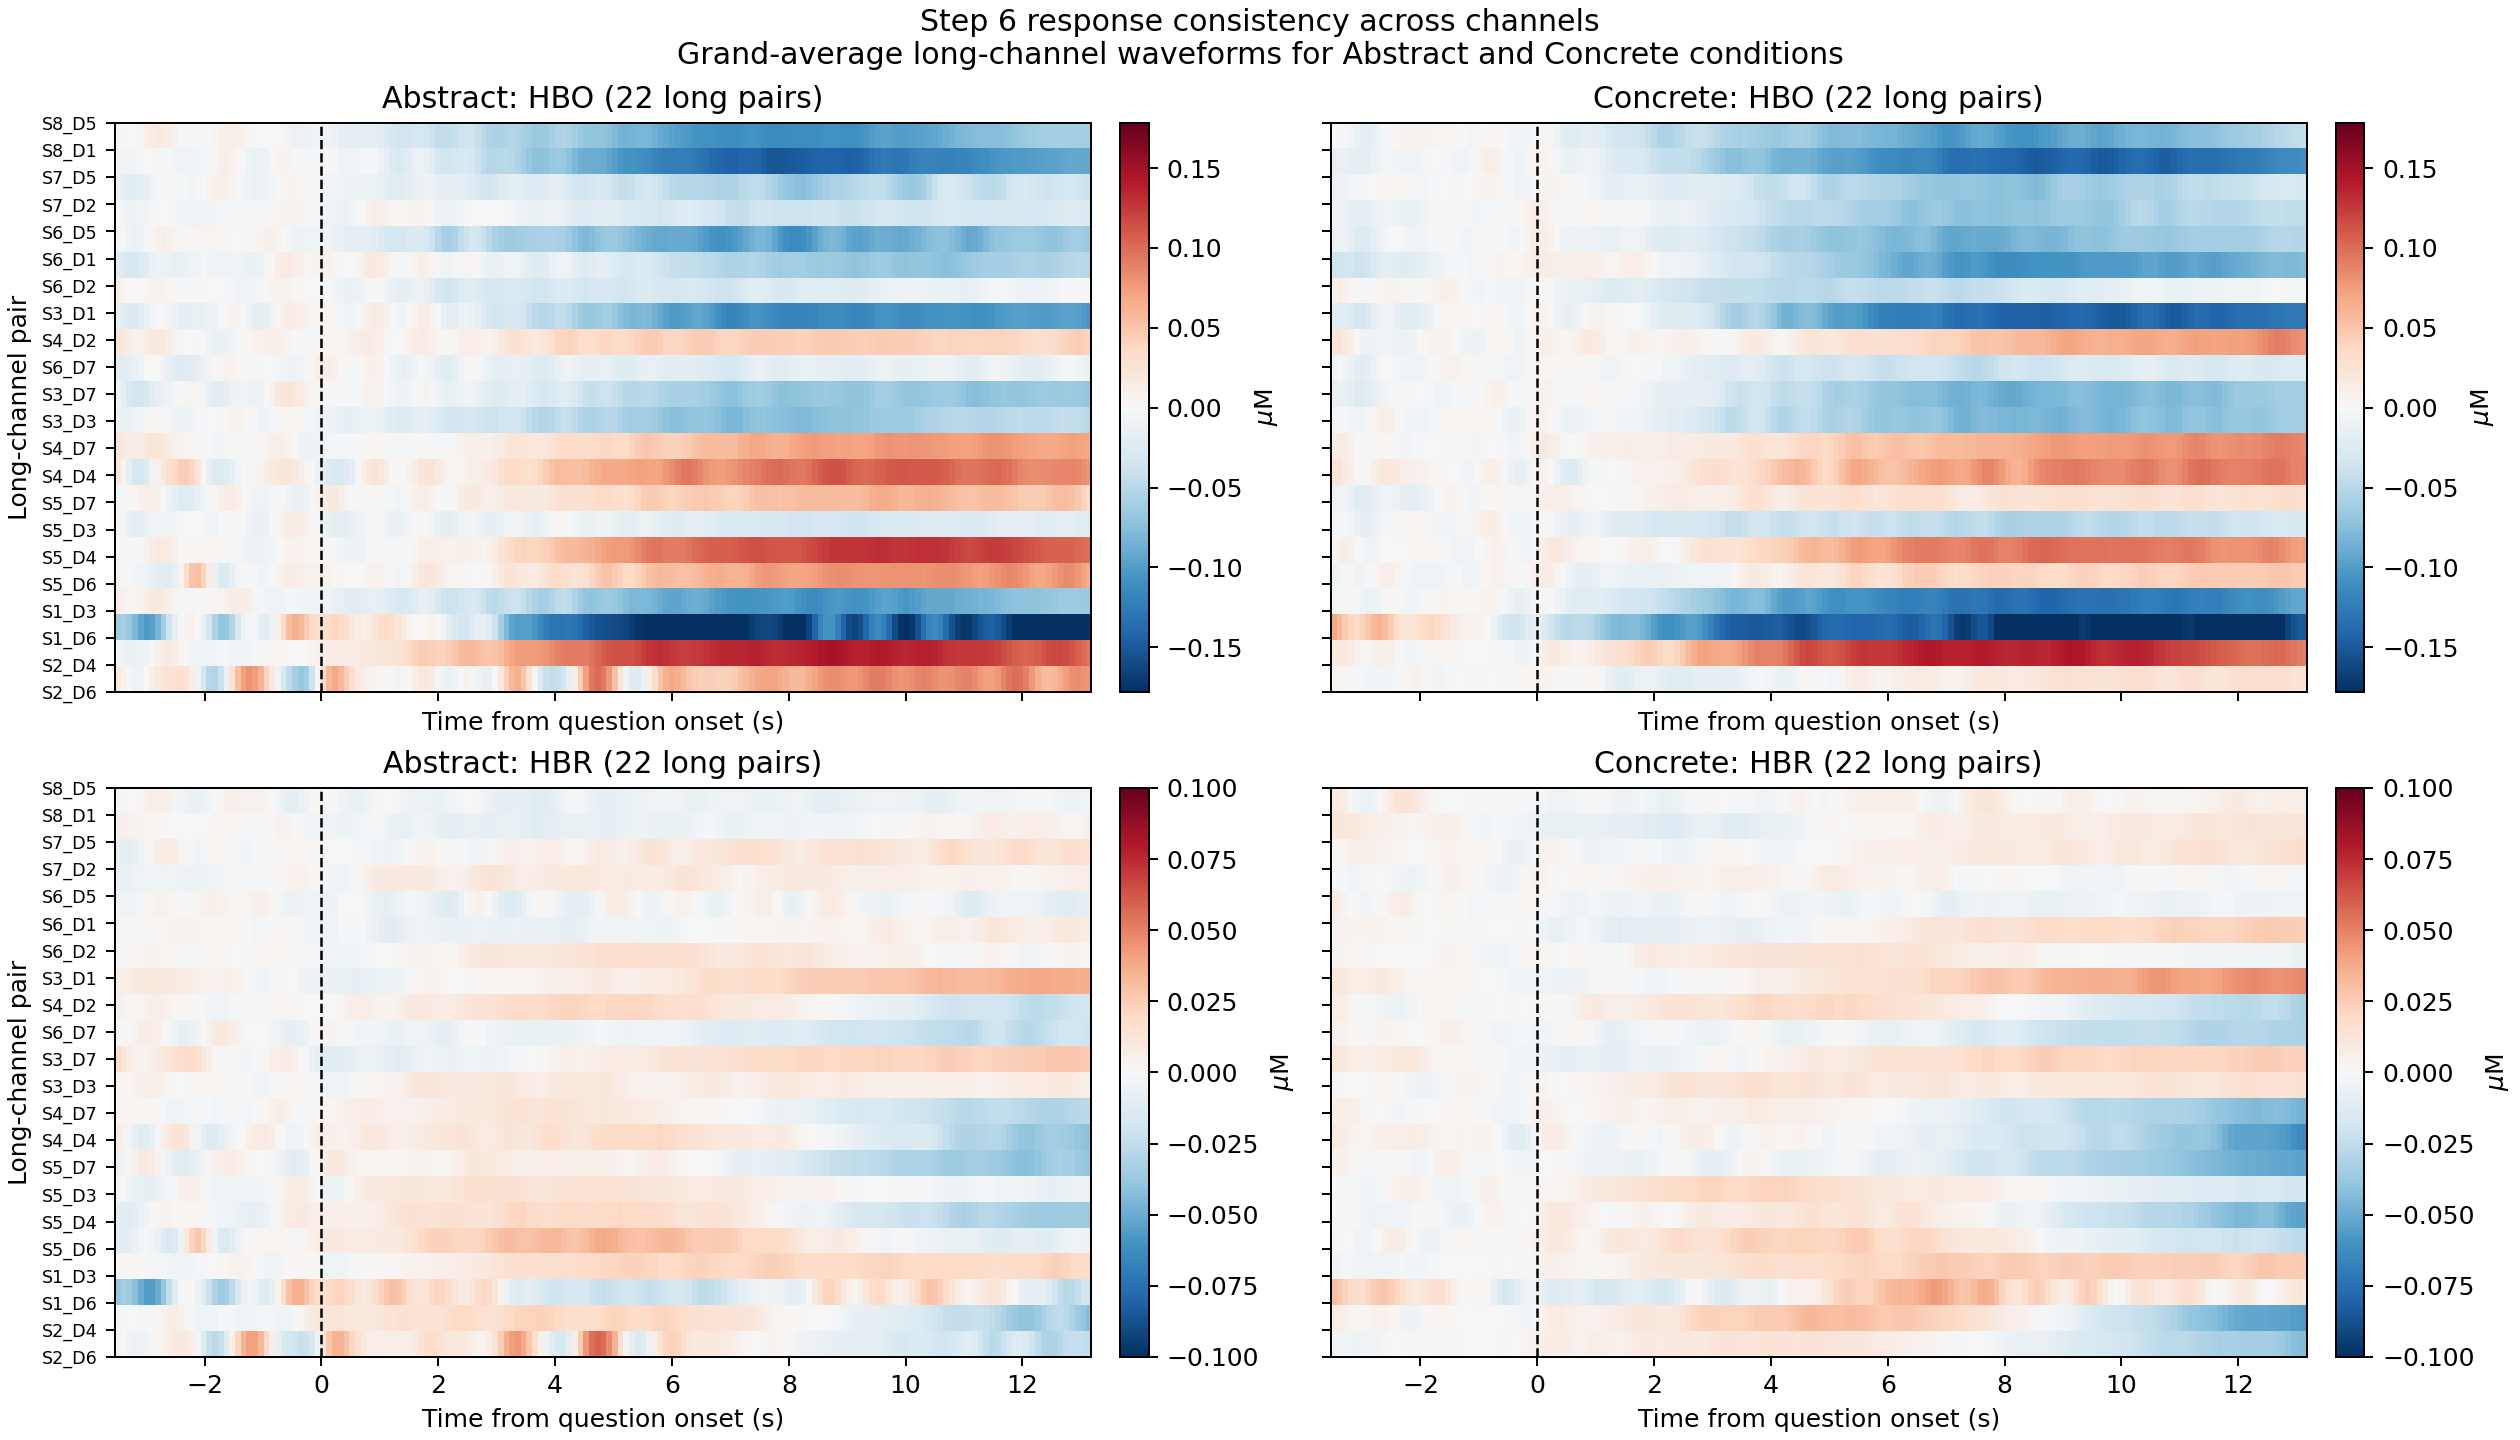
\includegraphics[width=0.95\linewidth]{../../figures/step6_visualization/channel_consistency_grid.png}
\caption{Grand-average long-channel response images across channels for the Abstract and Concrete conditions.}
\end{figure}
\begin{figure}[H]
\centering
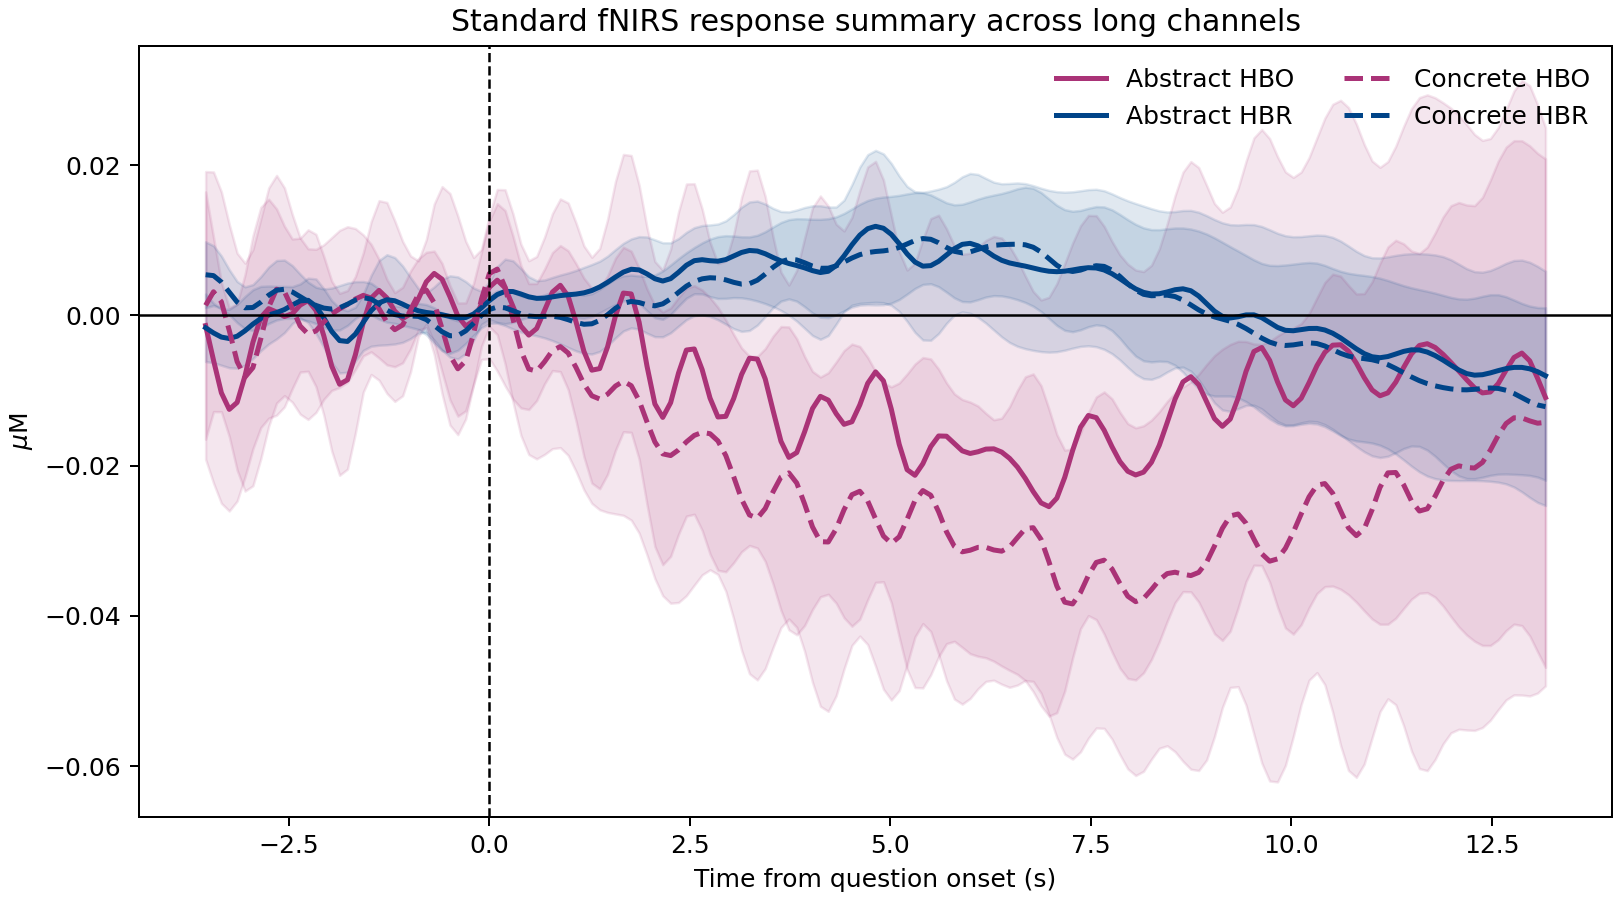
\includegraphics[width=0.92\linewidth]{../../figures/step6_visualization/standard_fnirs_compare.png}
\caption{Standard fNIRS waveform comparison across long channels for the Step~6 trial set.}
\end{figure}
\begin{figure}[H]
\centering
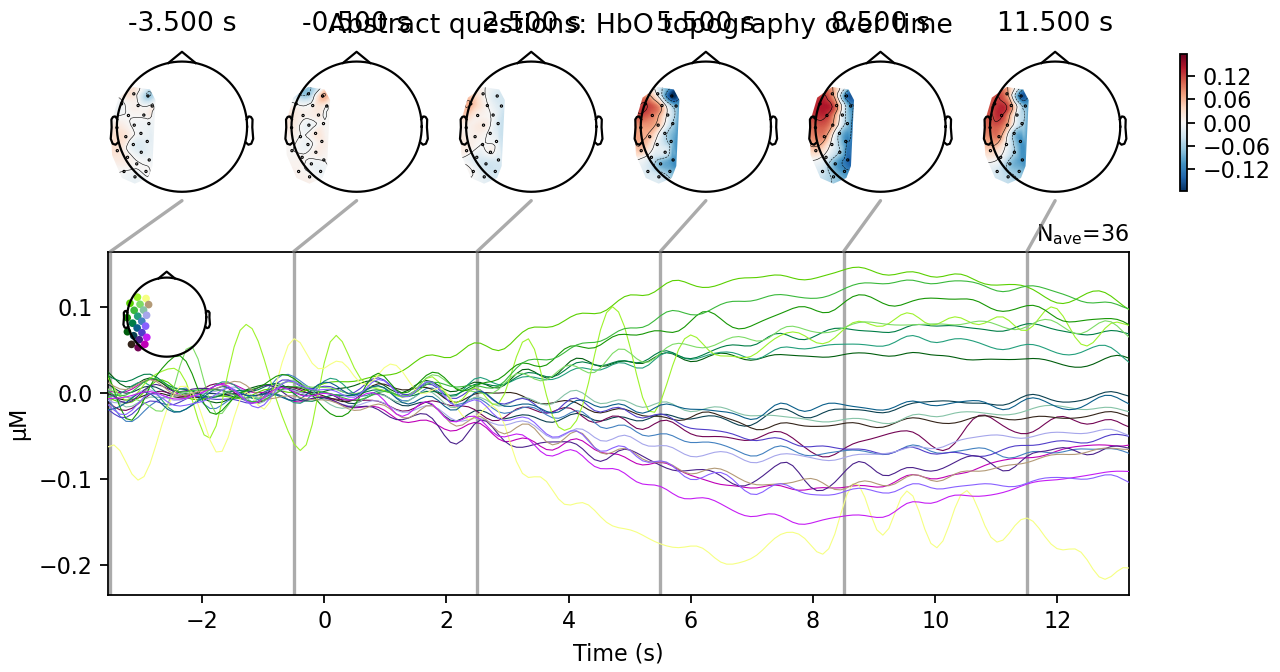
\includegraphics[width=0.95\linewidth]{../../figures/step6_visualization/abstract_hbo_joint.png}
\caption{Grand-average HbO topography over time for Abstract questions using the Step~6 included trial set.}
\end{figure}
\begin{figure}[H]
\centering
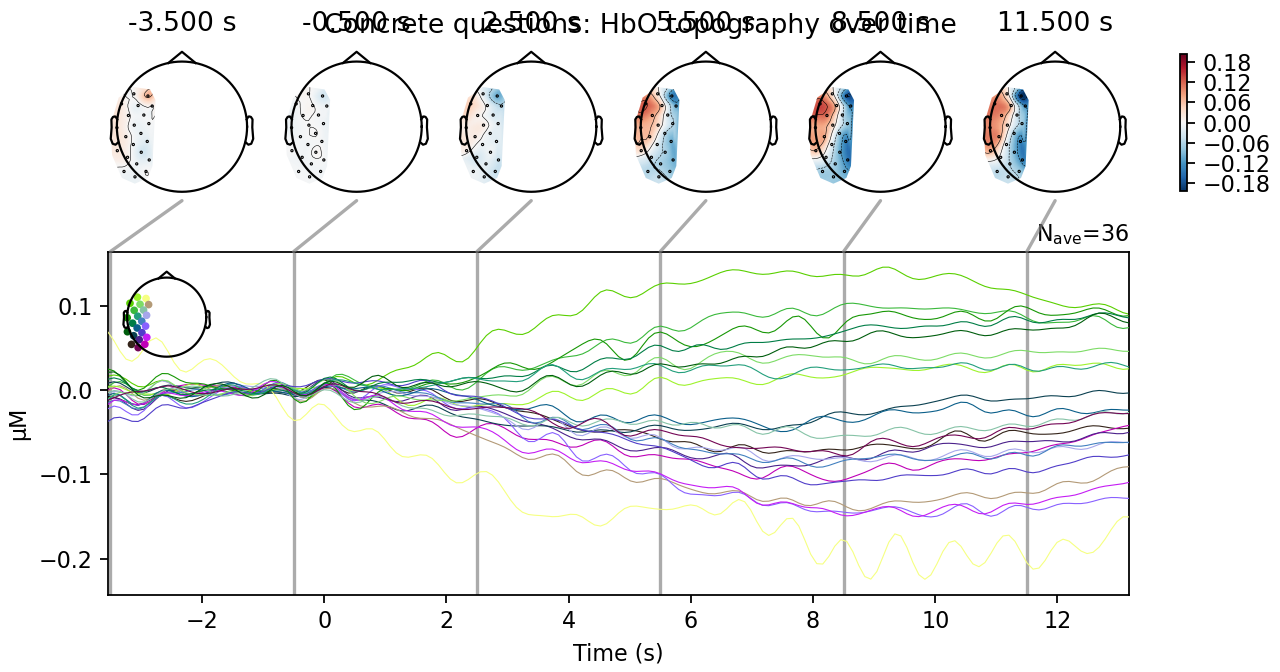
\includegraphics[width=0.95\linewidth]{../../figures/step6_visualization/concrete_hbo_joint.png}
\caption{Grand-average HbO topography over time for Concrete questions using the Step~6 included trial set.}
\end{figure}
\begin{figure}[H]
\centering
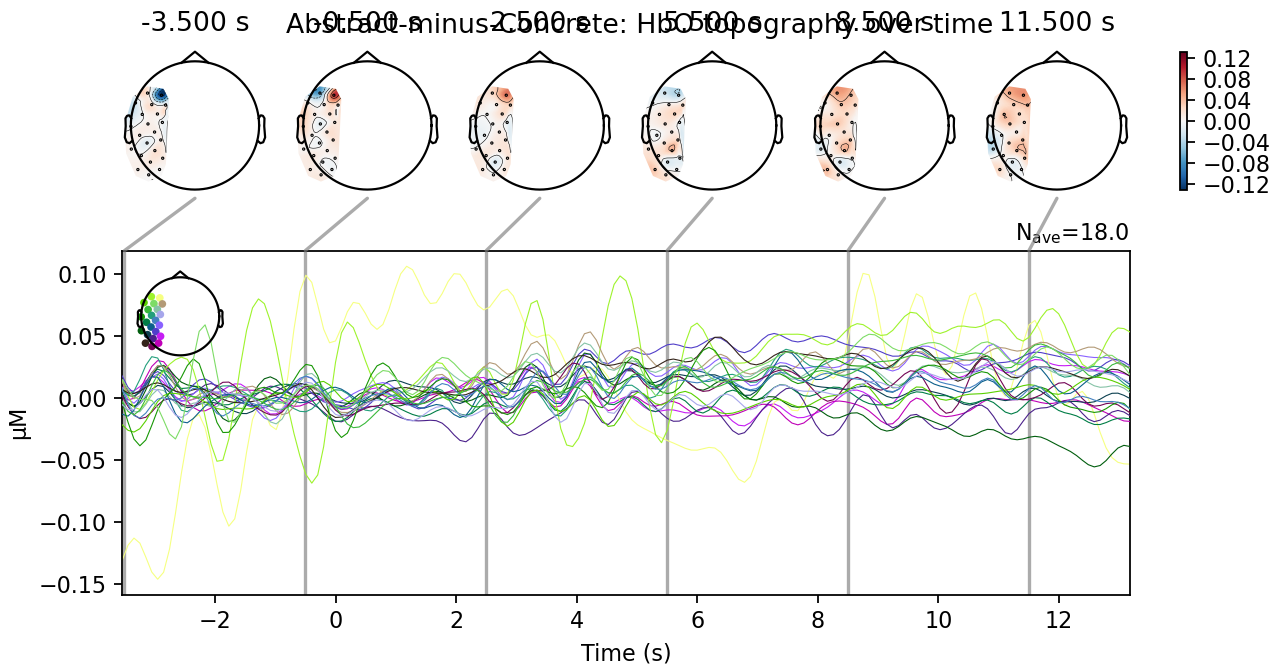
\includegraphics[width=0.95\linewidth]{../../figures/step6_visualization/abstract_minus_concrete_hbo_joint.png}
\caption{Grand-average Abstract-minus-Concrete HbO topography over time.}
\end{figure}
\begin{figure}[H]
\centering
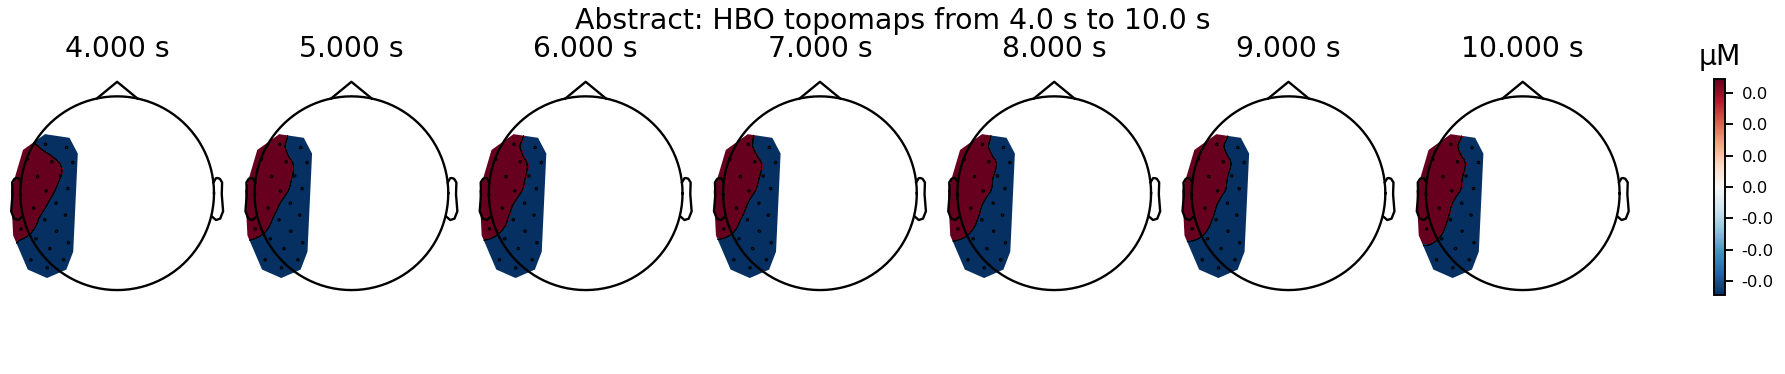
\includegraphics[width=0.48\linewidth]{../../figures/step6_visualization/abstract_hbo_topomap_series.png}
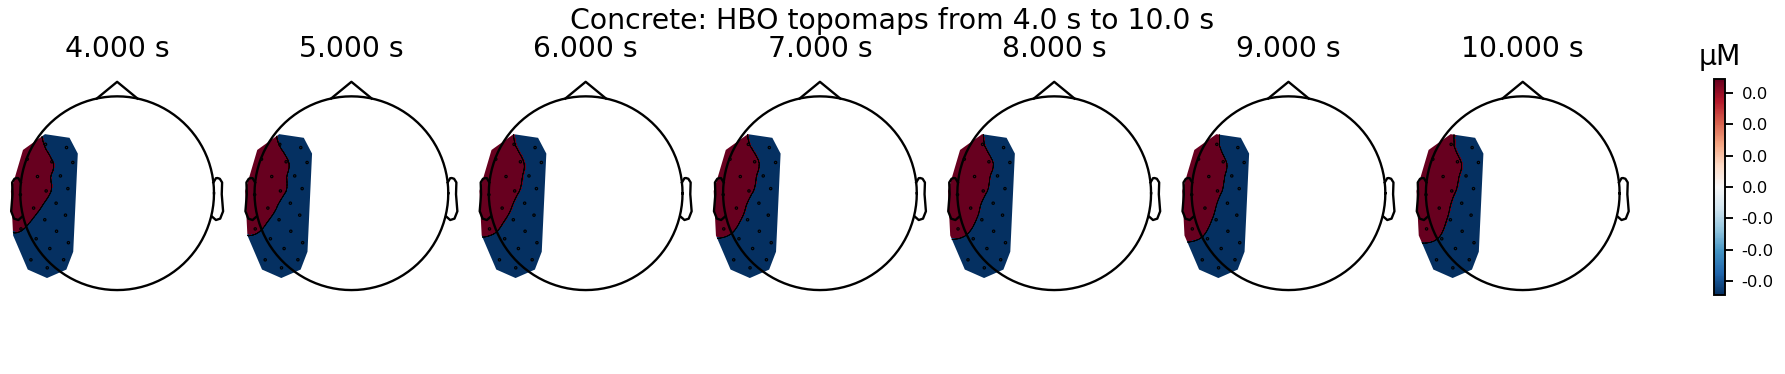
\includegraphics[width=0.48\linewidth]{../../figures/step6_visualization/concrete_hbo_topomap_series.png}
\caption{HbO topographic time series from 4.0~s to 10.0~s for the Abstract and Concrete conditions.}
\end{figure}
\begin{figure}[H]
\centering
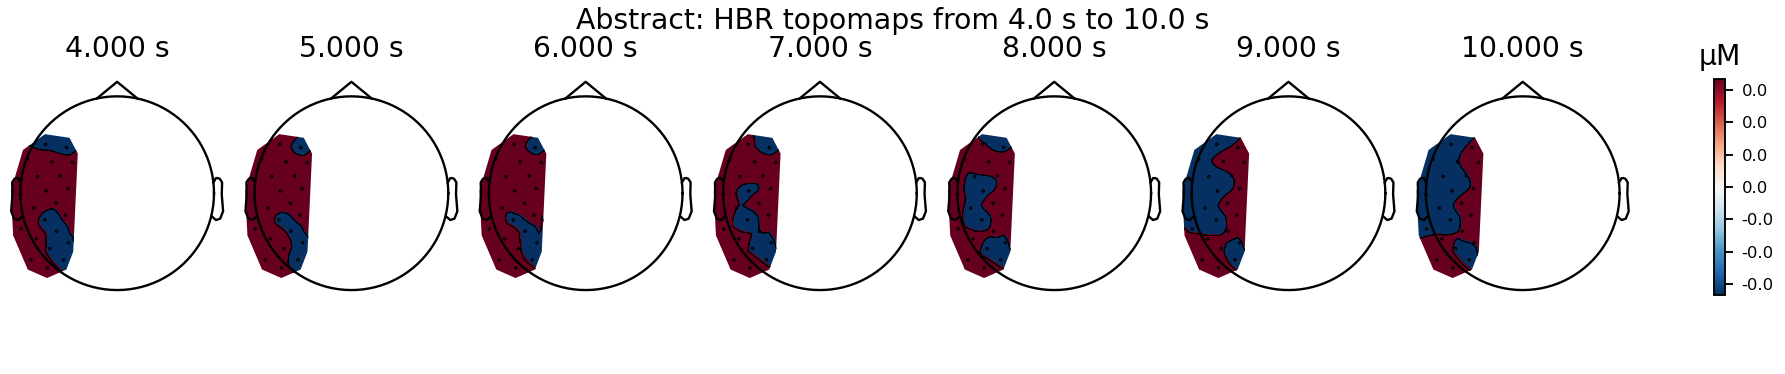
\includegraphics[width=0.48\linewidth]{../../figures/step6_visualization/abstract_hbr_topomap_series.png}
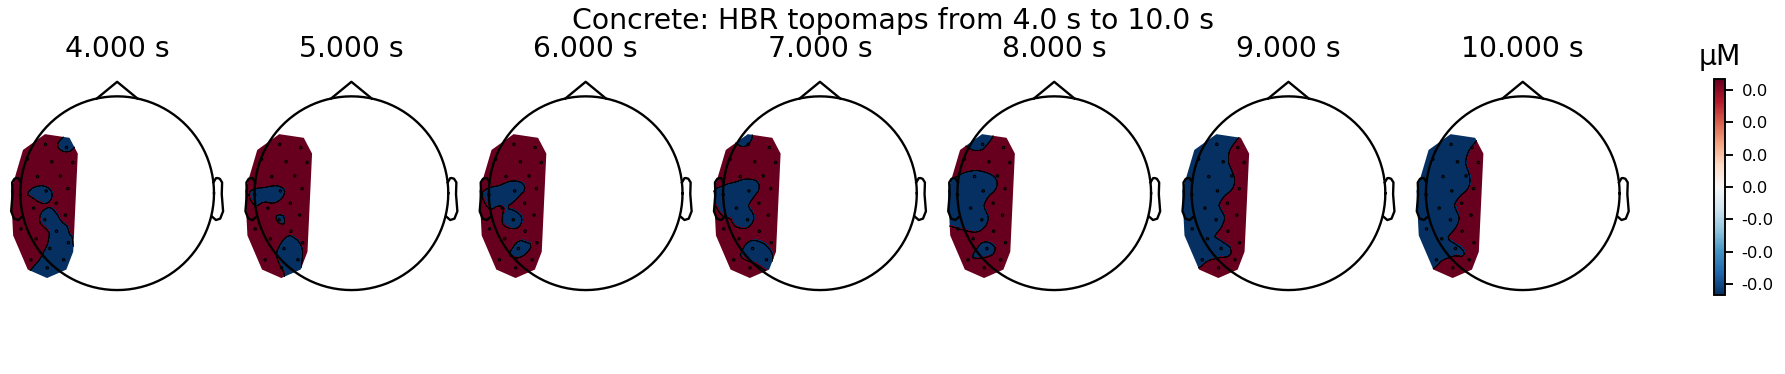
\includegraphics[width=0.48\linewidth]{../../figures/step6_visualization/concrete_hbr_topomap_series.png}
\caption{HbR topographic time series from 4.0~s to 10.0~s for the Abstract and Concrete conditions.}
\end{figure}
\begin{figure}[H]
\centering
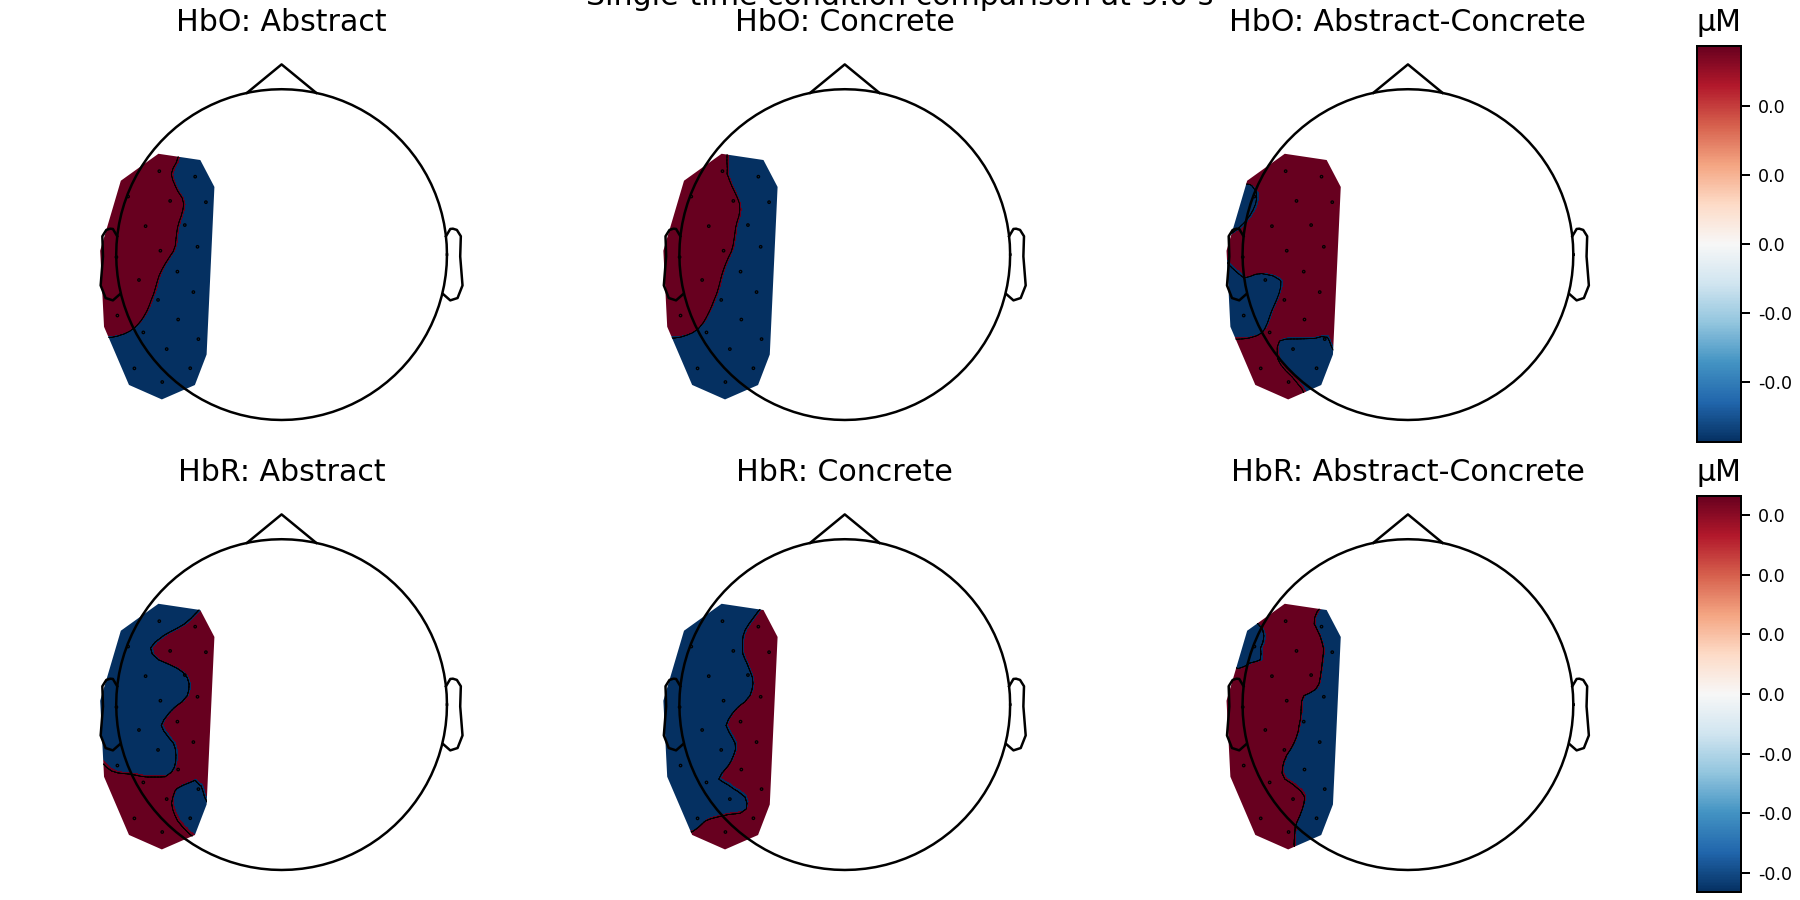
\includegraphics[width=0.95\linewidth]{../../figures/step6_visualization/abstract_concrete_single_time_comparison.png}
\caption{Single-time comparison at 9.0~s for Abstract, Concrete, and Abstract-minus-Concrete topographies for both HbO and HbR.}
\end{figure}
\begin{figure}[H]
\centering
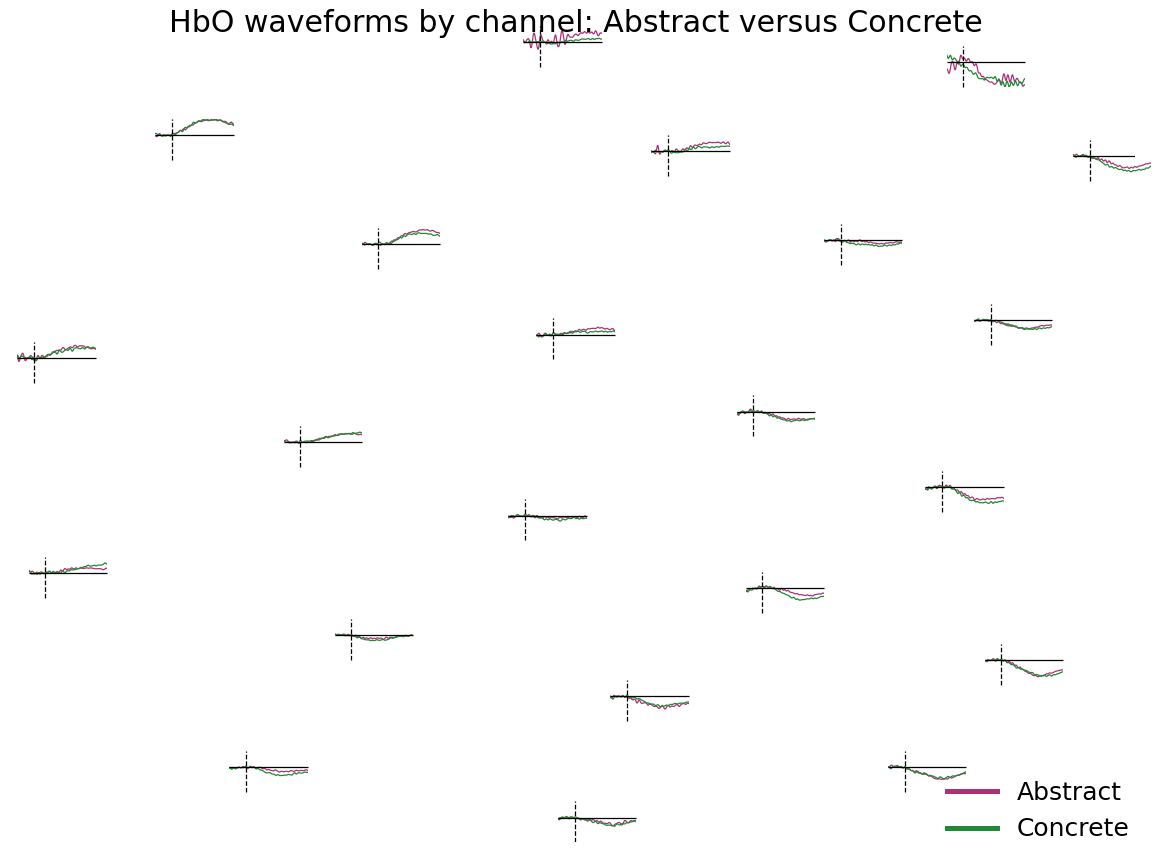
\includegraphics[width=0.95\linewidth]{../../figures/step6_visualization/abstract_concrete_hbo_evoked_topo.png}
\caption{HbO waveforms by long channel, overlaid for Abstract and Concrete, to show what drives the descriptive topographic differences.}
\end{figure}
\end{document}
